\newpage
\section*{Supplementary Information}
\subsection{Sampling routine}
Data gained from Molecular Dynamics (MD) and Markov Chain Monte Carlo processes (MD) are highly autocorrelated, thus we can not imply statistic developed for uncorrelated data. We have written a small in-house python package to calculate the expected value, the margin of error and effective sample size of correlated data.

The goal of the routine is to estimate mean and margins of error for an observable e.g. pressure, number of particles, end-to-end distance of a chain for a given confidence level or effective sample size. 

We also provided the way to limit sampling procedure with some timeout value. Our routine based on [] %[https://www.physik.uni-leipzig.de/~janke/Paper/nic10_423_2002.pdf]

There are multiple sampling routines developed for autocorrelated data, i.e. binning analysis, ... %some notes what others do

Expected value of the observable $X$ estimated as the mere mean of the sample $\overline{X}$, the same way one would do for uncorrelated data, whilst to estimate margins of error and \emph{effective} sample size $N_{eff}$ we used the next formulae. 
First of all we have to correct sample size to account that data is correlated:
\begin{eqnarray}
    N_{eff} = \frac{N}{2\tau}
    \\
    \tau  = \frac{1}{2} + \sum_{k=1}^{N} \text{acf} (k) (1-\frac{k}{N})
\end{eqnarray}
where $\tau$ is integrated autocorrelation time, $N$ size of autocorrelated data, $\text{acf} (k)$ is autocorrelation function on lag.

Note that ideally integral of  $\text{acf} (k)$ monotonically approaches some finite value, but due to unavoidable errors in number representation in computer and numeric integration methods it does not hold. 
For that reason instead of $\text{acf} (k)$ integral we use the maximum of its cumulative sum.

Margins of error (MOE) for a given confidence level $\gamma$ and effective sample size $N_{eff}$ is calculated using the next equation:
\begin{eqnarray}
    \text{MOE}(\gamma) = \frac{S_{N}}{\sqrt{N_{eff}}} t_{((1+\gamma)/2, N_{eff}-1)}
\end{eqnarray}
where $t_{(\alpha, \nu)}$ is percentile function (inverse cumulative distribution function) of Student’s distribution with $\nu$ degrees of freedom for $\alpha$ percentile,
$S_N$ is standard deviation of the sample.

The true mean of the observable $\mu_X$ lies inside the confidence interval with the confidence level $\gamma$.
\begin{equation}
    \Pr(\overline{X} - MOE(\gamma) \leq \mu_X \leq \overline{X} + MOE(\gamma)) = \gamma
\end{equation}

In our study we set $\gamma = 0.95$


\subsubsection{Routine implementation details}
%Probably we don't need this section

The arguments of our sampling routine are a function to calculate next sample and one of the next arguments: margins of error, effective sample size and timeout.

An observable is sampled in a loop till one of required targets is met (timeout, the margins of error or sample size). 
In the each following iteration of the loop, mean value and the margins of error are calculated with ever increasing precision and sample size. 

The loop follows the next steps:
\begin{itemize}
    \item Sample new data to double the sample size
    \item Recalculate $\tau$, $N_{eff}$, MOE
    \item If MOE is less, or $N_{eff}$ is bigger than desired, or run time exceed timeout exit loop
\end{itemize}

The routine returns mean of the sample, margins of error that defines confidence interval where true mean of distribution lies and \emph{effective} sample size that accounts that data is autocorrelated.

The routine is also described in Figure \ref{fig: sampling_diagram}

\begin{figure*}[t]
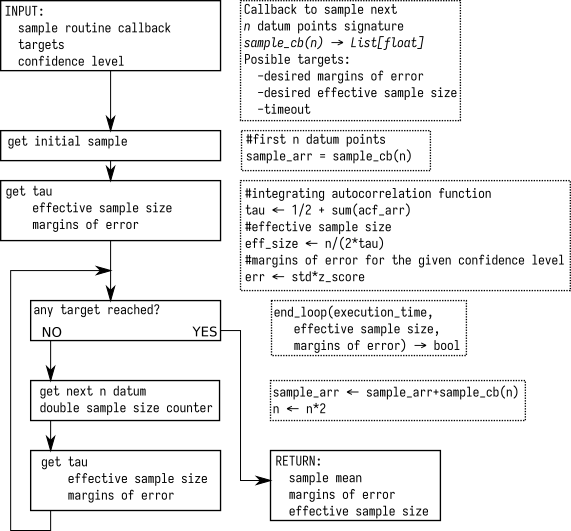
\includegraphics[width = 0.9\textwidth]{figures/sample_to_target_scheme.png}
\caption{Sampling routine diagram}
\label{fig: sampling_diagram}
\end{figure*}

\subsection{Monte Carlo process}
\subsubsection{Open system}
Free energy in grand-cannonical ensemble
\begin{equation}
\Omega = E-TS + \mu N 
\end{equation}
where $S$ is the entropy. Boltzman formula
\begin{equation}
S= k_B \ln \frac{V^N}{N!}
\end{equation}
The change of free energy associated with insertion ($\xi=1$) or deletion ($\xi=-1$) a particle is
\begin{equation}
\Delta \Omega =\kT\ln\left(V^{\xi}\frac{N!}{ (N+\xi)!}\right)+\xi\mu+\Delta E
\end{equation}
\subsubsection{Closed system}
In closed system ion pairs are exchanged between two finite volume boxes.

\begin{equation}
    \na_{I} + \cl_{I} \leftrightarrows \na_{II} + \cl_{II}
\end{equation}

Suppose an ion pair has been moved from box to another, then the change in entropy can be expressed as
\begin{eqnarray}
    \Delta S = 2 \log \left(\frac{V^{I}}{V^{II}} \right) ^ {\gamma}  \left(\frac{(N_{Na^{+}}^{I}+\mathcal{H}(\gamma))(N_{Cl^{-}}^{I}+\mathcal{H}(\gamma))}{(N_{Na^{+}}^{II}+\mathcal{H}(-\gamma))(N_{Cl^{-}}^{II}+\mathcal{H}(-\gamma))}\right)^{-\gamma}
\end{eqnarray}
where $\gamma$ defines the direction of the trial move, so that $\gamma_{I \rightarrow II} = -1$ when an ion pair moved from box I to box II and  $\gamma_{II \rightarrow I} = 1$ otherwise, $\mathcal{H}$ is the Heaviside step function.

The probability that the move will be accepted is calculated from the free energy change as
\begin{equation}
    \mathcal{P} = \exp(-\beta (\Delta E_{pot} - k_B T \Delta S))
\end{equation}

Thus, moving an ion pair from box I to box II change the entropy
\begin{equation}
    \Delta S_{I \rightarrow II} = 2 \log \left(\frac{V^{II}}{V^{I}} \right)  \frac{N_{Na^{+}}^{I} N_{Cl^{-}}^{I}}{(N_{Na^{+}}^{II}+1)(N_{Cl^{-}}^{II}+1)}
\end{equation}

The probability of this move ${I \rightarrow II}$ to be accepted

\begin{equation}
    \mathcal{P}_{I \rightarrow II} = \exp\left(-\beta (\Delta E_{pot} - 2 k_B T \log \left(\frac{V^{II}}{V^{I}} \right)  \frac{N_{Na^{+}}^{I} N_{Cl^{-}}^{I}}{(N_{Na^{+}}^{II}+1)(N_{Cl^{-}}^{II}+1)})\right)
\end{equation}

\begin{itemize}
\item perform a move of a random ion pair 
    \begin{equation}
    \left(\na +\cl\right)^{I} \leftrightarrows\left(\na +\cl\right)^{II}
\end{equation}

\item accept if 
    \begin{equation}
    \mathrm{rand}(0,1] < \left(\frac{V^{II}}{V^{I}}\right)^{\xi}\prod_{i=Na,\ Cl}\frac{N^I_i!}{(N^I_i+\xi)!}\frac{N^{II}_i!}{(N^{II}_i+\xi)!}\exp(-\beta\Delta E_{pot})
\end{equation}
\end{itemize}


\subsection{Donnan equilibrium in finite volume reservoirs}
Before we can explore any system properties and collect data the system has to be equilibrated. To achieve this we perform equilibration routine consist of sequence of Molecular Dynamics and Monte Carlo steps.
%Here we describe our technique
The result of equilibration is stationary of any observable such as pressure, end-to-end distance for polymer chains and ion distribution between reservoirs. 

The success and the cost in terms of computational time for the equilibration process heavily depend on initial guess. In our case we initialize the system with ion distribution corresponds to Donnan equilibrium.

In closed system number of ions in the system is constant, so Donnan equilibrium can be formulated as follows
\begin{equation}
    \frac{\left(N_{pairs} - N_{Cl^{-}}^{(gel)}\right)^2}{V_{salt}^2} = \frac{N_{Cl^{-}}^{gel} (N^{{(gel)}}_{A^{-}} + N_{Cl^{-}}^{(gel)})}{V_{gel}^2}
\end{equation}
where $N^{{(gel)}}_{A^{-}}$ is number of fixed anions in the box with the gel \ie acetic groups in the polymer gel.
Solving this equation with respect to $N^{{(gel)}}_{A^{-}}$ gives us the distribution of the ions between two boxes.

%probably not needed
\begin{eqnarray}
    %N_{Cl^{-}}^{(gel)} = \frac{\frac{N^{{(gel)}}_{A^{-}} V_{salt}^{2}}{2} + N_{pairs} V_{gel}^{2} - \frac{V_{salt} \sqrt{N^{{(gel)}}_{A^{-}}^{2} V_{salt}^{2} + 4 N^{{(gel)}}_{A^{-}} N_{pairs} V_{gel}^{2} + 4 N_{pairs}^{2} V_{gel}^{2}}}{2}}{V_{gel}^{2} - V_{salt}^{2}}
    \\
    N_{Na^{+}}^{(gel)} = N^{{(gel)}}_{A^{-}} + N_{Cl^{-}}^{(gel)}
    \\
    N_{Cl^{-}}^{(salt)} = N_{Na^{+}}^{(gel)} = N_{pairs} - N_{Cl^{-}}^{(gel)}
\end{eqnarray}